

% !TEX root = ../main.tex
% !TEX spellcheck = en_GB
% !TEX encoding = UTF-8 Unicode
% !TEX program = pdflatex
% !TEX options = -shell-escape

In Sect.~\ref{sec:CentralValue} and~\ref{sec:Covariance} we obtained some simplified expressions 
for the mean and the covariance of the trained networks under the assumption that the fluctuations
of the evolution operators $U(t)$ and |$V(t)$ are independent of the fluctuations of the networks 
at initialization. Here we quantify this assumption by computing these correlations explicitly 
for the dataset and architectures used in this work. In the absence of general theorems, it is necessary 
to verify the validity of these assumptions case by case. 

\begin{figure}[t!]
  \label{fig:xT3_exp_val}
  \centering
  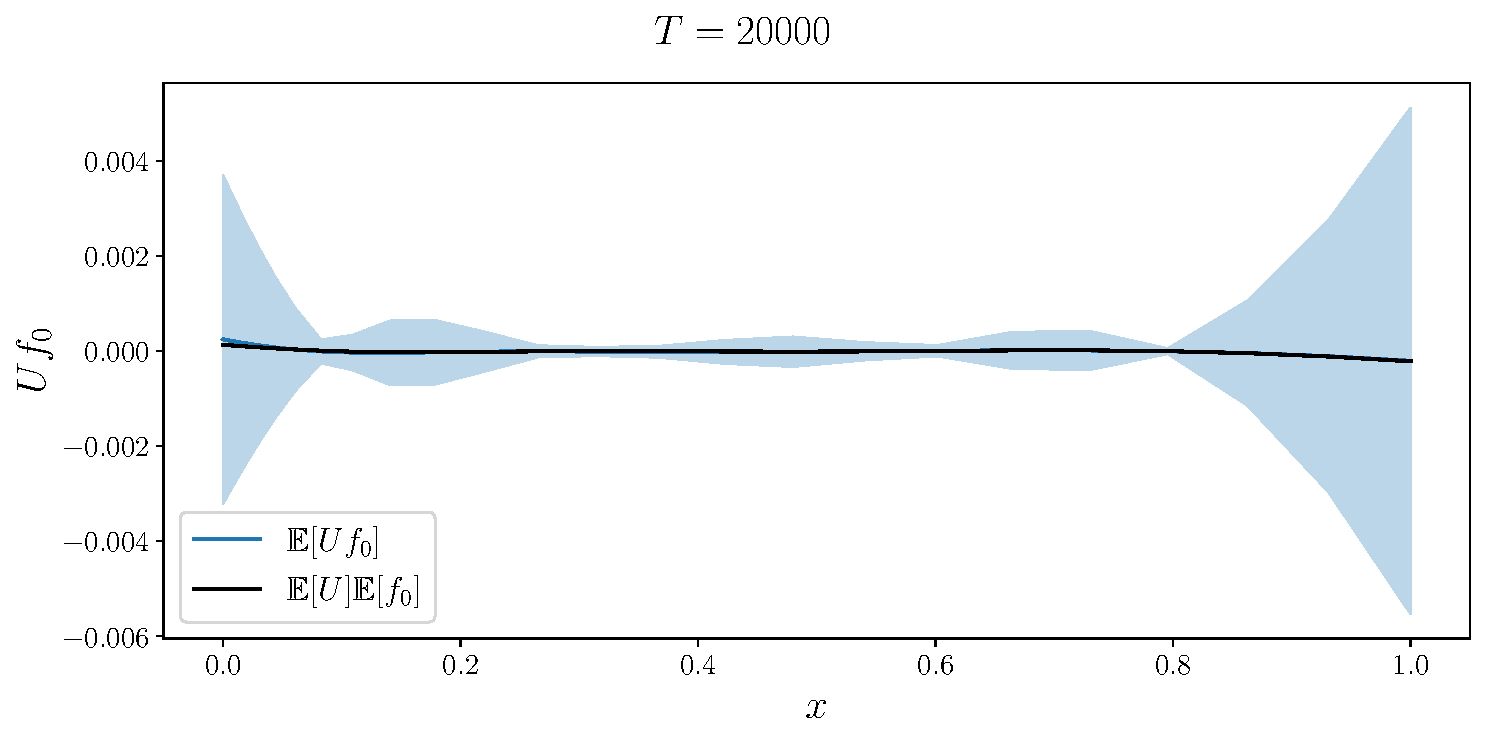
\includegraphics[width=0.65\textwidth]{plots/u_v_studies/u_f0_independence_20000_L0.pdf}
  \caption{Comparison of $\mathbb{E}\left[U(t) f_{0}\right]$ and $\bar{U}(t) \bar{f}_{0}$ as defined in 
    Eqs.~\eqref{eq:MeanValAtT} and~\eqref{eq:MeanValAtTNoCorr} respectively. 
    The data is obtained by choosing the frozen NTK at $T_{\rm
    ref} = 20000$, while $f_0$ is an ensemble of networks at initialisation
    (\textit{i.e.}\ $\mathbb{E}[f_0]=0$). The analytical solution is evolved for
    $T=20000$ epochs. L0 data is used.}
\end{figure}
% ===================================
